\documentclass{standalone}
\usepackage{tikz}
\usetikzlibrary{arrows}
\begin{document}

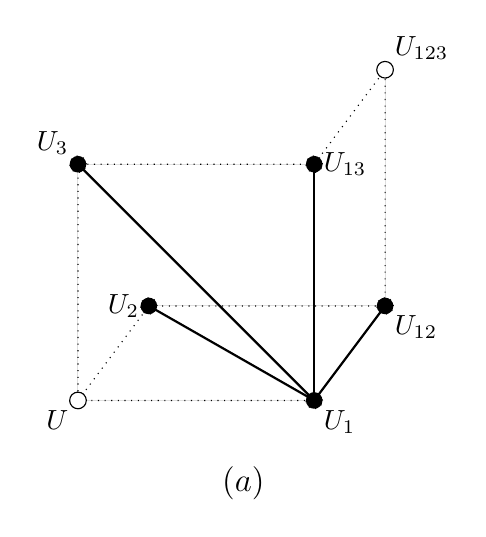
\begin{tikzpicture}[scale=1.5]
\node at (1.4,-.7) {\large $(a)$};

\draw[fill=black,dotted]
(2,0) circle(2pt) node[below right] {$U_1$} --
(2,2) circle(2pt) node[right] {$U_{13}$} --
(0,2) circle(2pt) node[above left] {$U_3$} --
(0,0) circle(2pt) node[below left] {$U$} -- (2,0);

\begin{scope}[xshift=6mm,yshift=8mm]
\draw[fill=black,dotted]
(0,0) circle(2pt) node[left] {$U_2$} -- 
(2,0) circle(2pt) node[below right] {$U_{12}$} --
(2,2) circle(2pt) node[above right] {$U_{123}$};
\end{scope}

\draw[dotted] (0,0) -- (.6,.8);
\draw[dotted] (2,0) -- (2.6,.8);
\draw[dotted] (2,2) -- (2.6,2.8);


\draw (0,0) circle(2pt)[fill=white];
\draw (2.6,2.8) circle(2pt)[fill=white];

\draw[thick] (2,0) -- (2.6,.8);
\draw[thick] (2,0) -- (2,2);
\draw[thick] (2,0) -- (0,2);
\draw[thick] (2,0) -- (.6,.8);
\end{tikzpicture}

\hspace{1cm}

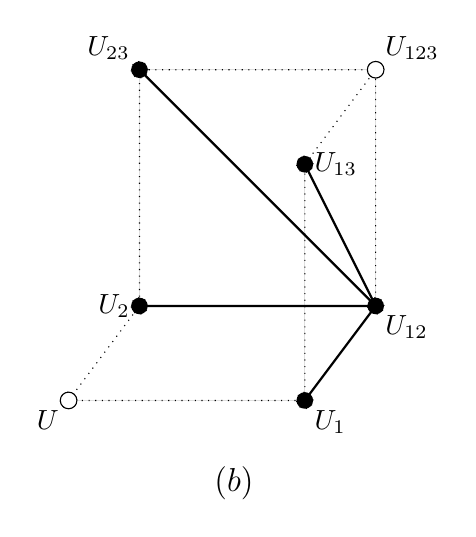
\begin{tikzpicture}[scale=1.5]
\node at (1.4,-.7) {\large $(b)$};

\draw[fill=black,dotted]
(0,0) circle(2pt) node[below left] {$U$} --
(2,0) circle(2pt) node[below right] {$U_1$} --
(2,2) circle(2pt) node[right] {$U_{13}$};

\begin{scope}[xshift=6mm,yshift=8mm]
\draw[fill=black,dotted]
(2,0) circle(2pt) node[below right] {$U_{12}$} --
(2,2) circle(2pt) node[above right] {$U_{123}$} --
(0,2) circle(2pt) node[above left] {$U_{23}$} --
(0,0) circle(2pt) node[left] {$U_2$} -- (2,0);
\end{scope}

\draw[dotted] (0,0) -- (.6,.8);
\draw[dotted] (2,0) -- (2.6,.8);
\draw[dotted] (2,2) -- (2.6,2.8);


\draw (0,0) circle(2pt)[fill=white];
\draw (2.6,2.8) circle(2pt)[fill=white];

\draw[thick] (2,0) -- (2.6,.8) -- (2,2);
\draw[thick] (.6,.8) -- (2.6,.8) -- (.6,2.8);
\end{tikzpicture}


\end{document}